% ------------------------------------------------------------------------------
% TYPO3 Version 9.4 - What's New (French Version)
%
% @license	Creative Commons BY-NC-SA 3.0
% @link		https://typo3.org/help/documentation/whats-new/
% @language	French
% ------------------------------------------------------------------------------


\section{Introduction}
\begin{frame}[fragile]
	\frametitle{Introduction}

	\begin{center}\huge{Introduction}\end{center}
	\begin{center}\huge{\color{typo3darkgrey}\textbf{Les faits}}\end{center}

\end{frame}

% ------------------------------------------------------------------------------
% TYPO3 Version 9.4 - The Facts

\begin{frame}[fragile]
	\frametitle{Introduction}
	\framesubtitle{TYPO3 Version 9.4 - Les faits}

	\begin{itemize}
		\item Date de sortie~: 4 septembre 2018
		\item Type de sortie~: Sprint Release
	\end{itemize}

	\begin{figure}
		
\includegraphics[width=0.95\linewidth]{Introduction/typo3-v94-banner.jpg}
	\end{figure}

\end{frame}

% ------------------------------------------------------------------------------
% System Requirements

\begin{frame}[fragile]
	\frametitle{Introduction}
	\framesubtitle{Prérequis système}

	\begin{itemize}
		\item PHP version 7.2 ou ultérieur
		\item Configuration PHP~:

			\begin{itemize}
				\item \texttt{memory\_limit} >= 256M
				\item \texttt{max\_execution\_time} >= 240s
				\item \texttt{max\_input\_vars} >= 1500
				\item L'option de compilation \texttt{-}\texttt{-disable-ipv6} \underline{NE} doit \underline{PAS} être utilisée
			\end{itemize}

		\item La majorité des serveurs de base de données supportés par \textbf{Doctrine DBAL} fonctionnent pour TYPO3.
			Les moteurs testés sont par exemple~:
	\end{itemize}

	\begin{figure}
		
\includegraphics[width=0.80\linewidth]{Introduction/logo-databases.png}
	\end{figure}

\end{frame}

% ------------------------------------------------------------------------------
% Development, Release and Maintenance Timeline

\begin{frame}[fragile]
	\frametitle{Introduction}
	\framesubtitle{Chronologie des développements, sorties et maintenances}

	\textbf{TYPO3 v9}

	\begin{figure}
		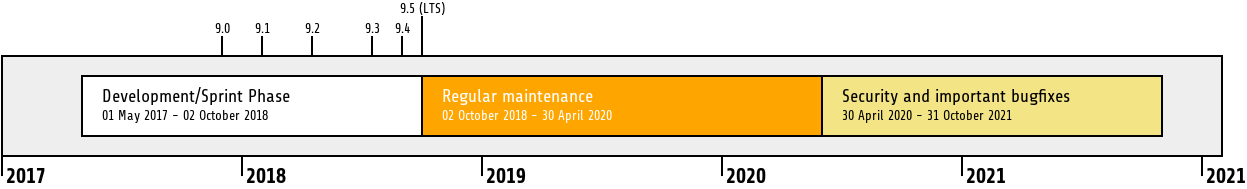
\includegraphics[width=1\linewidth]{Introduction/typo3-v9-lifecycle.png}
	\end{figure}

	\textbf{Support étendu}\newline
	\smaller
		\href{https://typo3.com}{TYPO3 GmbH} offre des options de support
		pour TYPO3 v9 LTS même après le 31 octobre 2021 pour deux ans
		supplémentaires maximum.
	\normalsize

%	\url{https://typo3.com/our-services/extended-support/}

\end{frame}

% ------------------------------------------------------------------------------
% TYPO3 v9 Roadmap

\begin{frame}[fragile]
	\frametitle{Introduction}
	\framesubtitle{Feuille de route TYPO3 v9}

	Dates de sortie prévues et axes principaux~:

	\begin{itemize}

		\item v9.0 \tabto{1.1cm}12/Déc./2017\tabto{3.4cm}Install Tool and Page Tree Refactoring,\newline
			\tabto{3.4cm}Unified Page Translations
		\item v9.1 \tabto{1.1cm}30/Jan./2018\tabto{3.4cm}Redirect Handling
		\item v9.2 \tabto{1.1cm}10/Avr./2018\tabto{3.4cm}Site Handling
        \item v9.3 \tabto{1.1cm}12/Juin/2018\tabto{3.4cm}SEO and URL Routing Preparations
		\item
			\begingroup
				\color{typo3orange}
                    v9.4 \tabto{1.1cm}04/Sep./2018\tabto{3.4cm}URL Routing for Pages
			\endgroup
		\item v9.5 \tabto{1.1cm}02/Oct./2018\tabto{3.4cm}LTS Release

	\end{itemize}

	\smaller
		\url{https://typo3.org/article/typo3-v9-roadmap/}\newline
		\url{https://typo3.org/cms/roadmap/}
	\normalsize

\end{frame}

% ------------------------------------------------------------------------------
% Installation

\begin{frame}[fragile]
	\frametitle{Introduction}
	\framesubtitle{Installation}

	\begin{itemize}
		\item Procédure officielle \textit{classique} d'installation sous Linux/Mac OS X\newline
			(DocumentRoot considéré \texttt{/var/www/site/htdocs})~:
		\begin{lstlisting}
$ cd /var/www/site
$ wget --content-disposition get.typo3.org/9.4
$ tar xzf typo3_src-9.4.0.tar.gz
$ cd htdocs
$ ln -s ../typo3_src-9.4.0 typo3_src
$ ln -s typo3_src/index.php
$ ln -s typo3_src/typo3
$ touch FIRST_INSTALL
		\end{lstlisting}

		\item Liens symboliques sous Microsoft Windows~:

			\begin{itemize}
				\item Utiliser \texttt{junction} sous Windows XP/2000
				\item Utiliser \texttt{mklink} sous Windows Vista, Windows 7 et supérieurs
			\end{itemize}

	\end{itemize}
\end{frame}

% ------------------------------------------------------------------------------
% Installation using composer

\begin{frame}[fragile]
	\frametitle{Installation et mise à jour}
	\framesubtitle{Installation avec \texttt{composer}}

	\begin{itemize}
		\item Installation avec \textit{composer} sous Linux, Mac OS X et Windows 10~:

			\begin{lstlisting}
$ cd /var/www/site/
$ composer create-project typo3/cms-base-distribution CmsBaseDistribution ^9
			\end{lstlisting}

		\item Alternativement, créez votre propre fichier \texttt{composer.json} et exécutez~:

			\begin{lstlisting}
$ composer install
			\end{lstlisting}

			Plus de détails et exemples de fichiers \texttt{composer.json} disponibles à~:\newline
			\smaller
				\href{https://composer.typo3.org}{https://composer.typo3.org}
			\normalsize

	\end{itemize}
\end{frame}

% ------------------------------------------------------------------------------
